\documentclass[a4paper,12pt]{article}

\title{Math 31 \\ Antiderivatives and Integration}
\author{Jad Chehimi}

% document setup
\renewcommand{\familydefault}{\sfdefault}
\linespread{1.25}
\usepackage[margin=1in]{geometry}
\usepackage{setspace}
\usepackage{enumitem}
\setlist{nosep}
\usepackage{color,soul}
\setcounter{secnumdepth}{0}

% tools
\usepackage[hidelinks]{hyperref}
\usepackage{float}
%% images
\usepackage{graphicx}
\graphicspath{ {./images/} }
%% science
\usepackage{siunitx}
\usepackage{physics}

\begin{document}
\maketitle

% temp
\begin{center}
\Huge
Unfinished!
\normalsize
\end{center}
% temp

\tableofcontents

\pagebreak

\section{Antiderivative}
The antiderivative is the opposite of a derivative.

\begin{itemize}
    \item{$F(x)$ = antiderivative}
    \item{$f(x)$ = original}
    \item{$f'(x)$ = derivative}
\end{itemize}

\subsection{C}
The derivative of any constant is zero. Therefore, even if the original function has no constant, it could have had it in the antiderivative.

This is accounted for by adding the constant variable $C$.
$$f(x) = 2x$$
$$F(x) = x^2 + C$$

\subsection{Antiderivative Tips}

\subsubsection{Polynomials}
\begin{itemize}
    \item{Deriving involves subtracting the exponent by 1}
    \item{Therefore, antideriving \hl{always} involves \hl{adding 1 to the exponent}}
    \item{Determine a coefficient for the antiderivative that, if derived, would equal the original
            \begin{itemize}
                \item{Keep the original coefficient}
                \item{Divide the term by the new exponent (after adding 1)}
                \item{Simplify}
                \item{e.g. $f(x) = 6x^2$\\$F(x) = 6x^3 = \frac{6x^3}{3} = 2x^3$}
                \item{$F(x) = 2x^3 + C$}
            \end{itemize}
        }
    \item{Imagine constants in the original function having $x^0$ on them. Therefore, the antiderivative of $-5$ would be $-5x$}
\end{itemize}

e.g.
$$f(x) = 8x, F(x) = x^8 + C$$
$$f(x) = 2x + 5, F(x) = x^2 + 5x + C$$
$$f(x) = 6x^3, F(x) = \frac{3}{2}x^4 + C$$
$$f(x) = 2x^2 - x + 7, F(x) = \frac{2}{3}x^3 - \frac{1}{2}x^2 + 7x + C$$

\subsection{Trigonometry with angle x}
Follow the normal trigonometry derivative rules, but just in reverse. These are also on your formula sheet.

$$f(x) = \cos{x} - \sin{x}$$
$$F(x) = \sin{x} + \cos{x} + C$$

\subsection{Trigonometry with angle ax}
For all trignometric functions, do the "reverse" derivative like the previous section.
To account for the coefficient, divide the term by the derivative of the trigonometric function's argument.

This is to get rid of the coefficient on the whole term if you derive $F(x)$, therefore making it correct.

$$f(x) = \cos{6x}$$
$$F(x) = \frac{1}{6}\sin{6x} + C$$

\subsection{Exponential Functions}
\begin{itemize}
    \item{Add 1 to the exponent}
    \item{Divide everything by the new exponent}
\end{itemize}

$$f(x) = \sqrt[3]{x} = x^{\frac{1}{3}}$$
$$F(x) = \frac{x^{\frac{4}{3}}}{\frac{4}{3}} = \frac{3}{4}x^{\frac{4}{3}} + C$$

\subsection{Variable in Denominator}
The following is in your formula sheet.
$$\dv{}{x}\ln{u} = \frac{1}{u} \cdot \dv{u}{x}$$
Using this, you can convert a fraction derivative into a natural log function antiderivative.

$$f(x) = \frac{-3}{x}, F(x) = -3\ln{x} + C$$
$$f(x) = \frac{2x}{x^2 + 1}, F(x) = \ln{(x^2 + 1)} + C$$

\subsection{Euler's Number}
\begin{itemize}
    \item{Divide everything by the derivative of the exponent}
\end{itemize}

$$f(x) = e^{3x}$$
$$F(x) = \frac{1}{3}e^{3x} + C$$

$$f(x) = xe^{x^2}$$
$$F(x) = \frac{xe^{x^2}}{2x} = \frac{1}{2}e^{x^2} + C$$

\subsection{Reciprocal Trigonometric Functions}
Like the derivatives of trig functions, the antiderivatives of trig functions is on your formula sheet under "INTEGRALS \& ANTIDERIVATIVES."

$$f(x) = \sin^2{x}\cos{x}$$
$$F(x) = \frac{1}{3}\sin^3{x} + C$$

\pagebreak

\section{Kinematics}
Recall that,
\begin{itemize}
    \item{$s$ = displacement}
    \item{$s'$ = $v$ = velocity}
    \item{$s''$ = $v'$ = $a$ = acceleration}
\end{itemize}
It works backwards as well with antiderivatives.

\section{Differential Equations with Initial Conditions}
When getting the antiderivative, you'll have the unknown value of C.

In questions with initial conditions, you can solve for C, then write the equation.

e.g. Solve for the differential equation $\dv{s}{t} = 2t$ with the initial conditions of $s = 3$ when $t = 0$
$$s(0) = 3, v(t) = 2t$$
$$s(t) = t^2 + C$$

$$s(0) = 3 = 0^2 + C, C = 3$$
$$s(t) = t^2 + 3$$

For questions that are related to kinematics, you will often need to start with \hl{acceleration due to gravity} ($a = \SI{9.81}{\m/\s^2}$)

Find the antiderivative of acceleration to get velocity and/or displacement. 

Solve for $C$ as you go by \hl{substituting values you know} from the question.

Eventually you'll have all the equations you'll need to answer the problem.

\pagebreak

e.g. A rock is thrown down a \SI{50}{\m} deep well with a velocity of \SI{20}{\m/\s}. How long will it take the rock to hit the bottom of the well? How fast will it be going at this time?

List what you know.

$a(t) = \SI{-9.81}{\m/\s^2}$, $v(0) = \SI{-20}{\m/\s}$, $s(0) = \SI{50}{\m}$

Find the equations you need.

$$a(t) = -9.81$$

$$v(t) = -9.81t + C$$
$$-20 = -9.81(0) + C$$
$$v(t) = -9.81t - 20$$

$$s(t) = -\frac{9.81}{2}t^2 - 20t + C$$
$$50 = -\frac{9.81}{2}(0)^2 - 20(0) + C$$
$$s(t) = -\frac{9.81}{2}t^2 - 20t + 50$$

Answer the question with your new equations.

Time for rock to hit the bottom.
$$0 = -\frac{9.81}{2}t^2 - 20t + 50$$
$$t = \SI{1.75}{\s}$$

How fast rock hit bottom.
$$v(1.75) = -9.81(1.75) - 20$$
$$v(1.75) = \SI{-37.2}{\m/\s}$$

More examples page 7-9 in booklet.

\pagebreak

\section{Integrals}
The integral of a curve function is the \hl{area under the curve}.

\subsection{Properties of Integrals}
$$\int_a^a{f(x)}dx = 0$$
$$\int^a_b{f(x)}dx = -\int^b_a{f(x)}dx$$
$$\int^a_b{c \cdot f(x)}dx = c\cdot\int^a_b{f(x)}dx$$
$$\int^a_b{\Big( f(x) \pm g(x) \Big)}dx = \int^a_b{f(x)} \pm \int^a_b{g(x)}$$

\subsection{Indefinite Integrals}
Indefinite integrals have no bounds, and are the same as antiderivatives.

Take the antiderivative of $f(x)$ with respect to $x$.
$$F(x) = \int{f(x)}dx$$

\subsection{Definite Integrals}
The definite integral from $a$ to $b$ is, which is the area under the curve between an interval/range of two $x$ points.
$$\int^a_b{f(x)}dx = F(a) - F(b)$$

\begin{itemize}
    \item{"Under the curve" being the area \hl{between the curve and the $x$-axis}}
    \item{\hl{$a$/top is the larger value, $b$/bottom is the smaller value. (typically)}}
\end{itemize}

Find $F(x)$, then substitute $F(x)$ with $a$ subtracting $b$. 

You can ignore the $C$, since both functions have it, it will always be cancelled out.

e.g. $$\int^3_1{(x)}dx = F(3) - F(1)$$
$$F(x) = \frac{1}{2}x^2 + C$$
$$(\frac{3^2}{2} + C) - (\frac{1^2}{2} + C)$$
$$-15 - (-6) = -9$$

\section{Area Under The Curve}
\subsection{Curve Is Positive (Above X-axis)}
Calculate the definite integral like normal.

\subsection{Curve Is Negative (Under X-axis)}
The area under the curve is negative when the area is under the x-axis. If you just get the area under the curve normally like above, this area would be subtracted from the total.

In order to properly get the area, you need to,
\begin{itemize}
    \item{Calculate the \hl{area above and below the x-axis separately} (split them up at x-intercept)}
    \item{Add the \hl{absolute value} of each of them together}
\end{itemize}

e.g. Determine the area under $y = 3x - x^2$ for $0 \leq x \leq 5$
\begin{figure}[H]
    \centering
    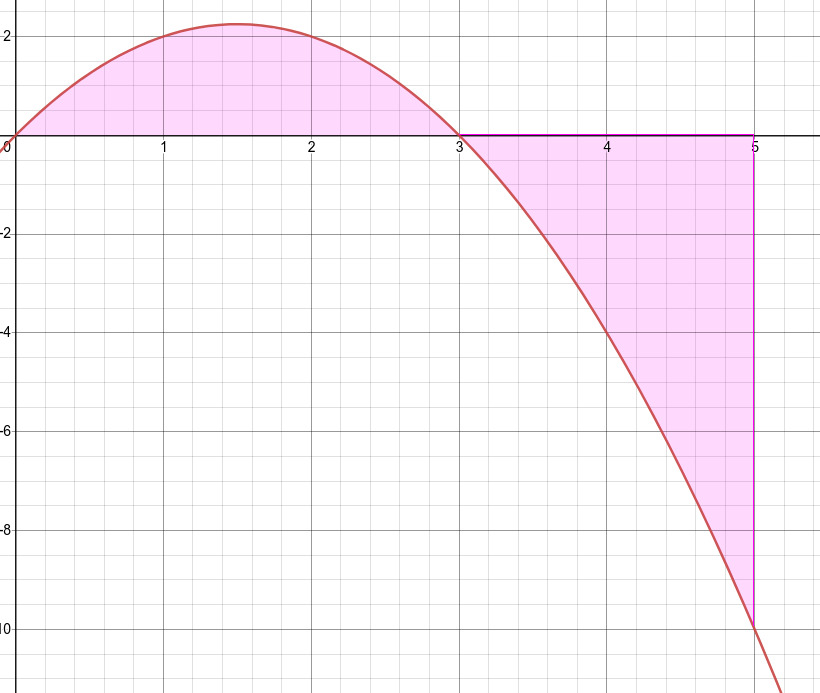
\includegraphics[width=0.75\textwidth]{negative}
\end{figure}
0-3 is positive, 3-5 is negative.

$$\abs{\int^3_1{(3x - x^2)}dx} + \abs{\int^5_3{(3x - x^2)}dx}$$

\pagebreak

\subsection{Areas Between Curves}
\begin{itemize}
    \item{Area of the curve on top minus the area of the curve below (top $-$ bottom)}
    \item{Combine the two integral formulas into one using properties of integrals (optional, but makes things easier)}
    \item{Some questions don't give the interval to calculate. In that case, find the intersections of the two curves (there should be two)}
\end{itemize}

e.g. \emph{Determine the area between $y = x^2 + 1$ and $y = x$ for $1 \leq x \leq 3$}
\begin{figure}[H]
    \centering
    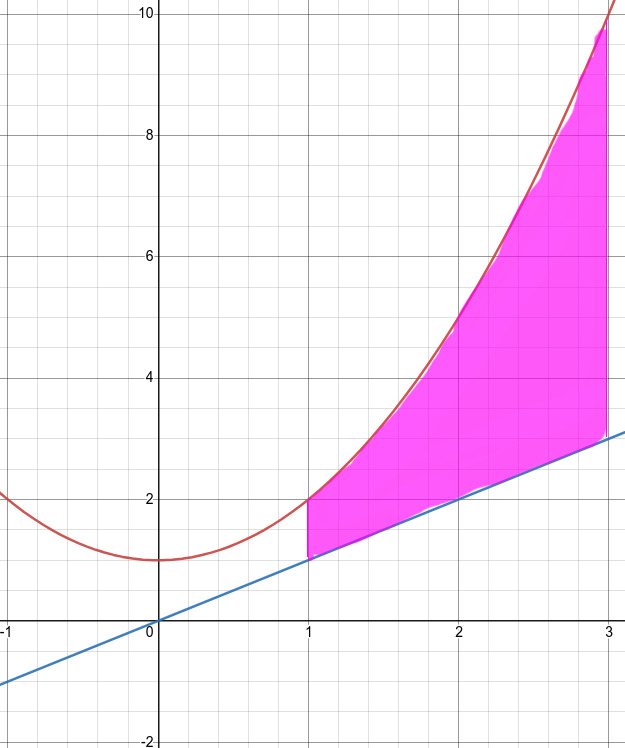
\includegraphics[width=0.50\textwidth]{between}
\end{figure}

$$\int^3_1{(x^2 + 1)}dx - \int^3_1{(x)}dx$$
$$\int^3_1{(x^2 + 1) - (x)}dx$$

\pagebreak

e.g. \emph{Determine the area between $y = x^2$ and $y = 2x - x^2$}
\begin{figure}[H]
    \centering
    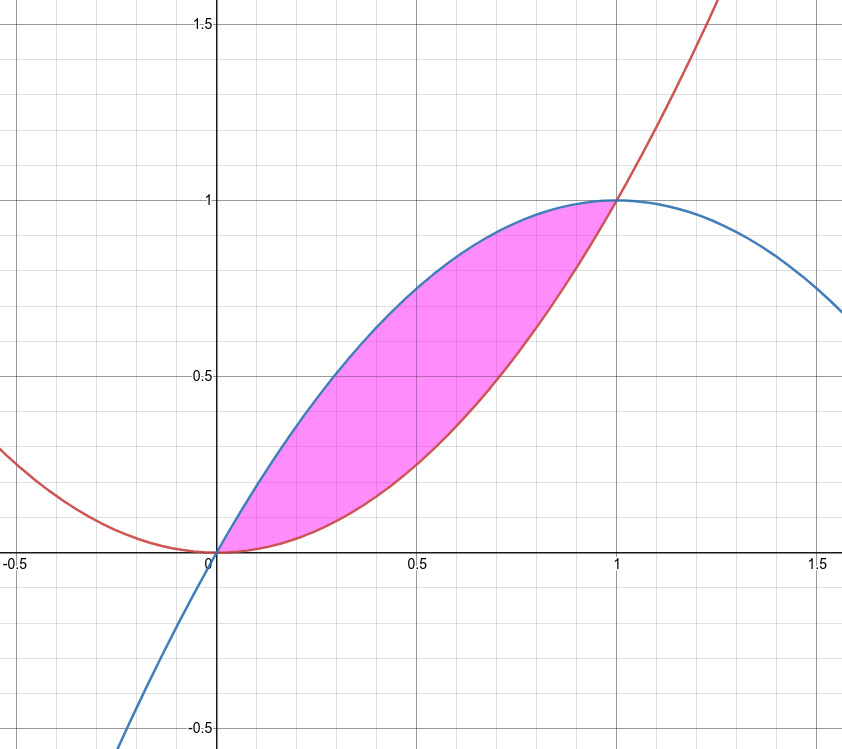
\includegraphics[width=0.75\textwidth]{between2}
\end{figure}
No intervals given, but intersects are $x = 0, 1$. (only part thats between curves)

$$\int^1_0{(2x - x^2)}dx - \int^1_0{(x^2)}dx$$
$$\int^1_0{(2x - 2x^2)}dx$$
$$F(x) = x^2 - \frac{2}{3}x^3 + C$$
$$F(1) - F(0) = \frac{1}{3}$$

\end{document}
